\documentclass[]{article}
\usepackage{lmodern}
\usepackage{amssymb,amsmath}
\usepackage{ifxetex,ifluatex}
\usepackage{fixltx2e} % provides \textsubscript
\ifnum 0\ifxetex 1\fi\ifluatex 1\fi=0 % if pdftex
  \usepackage[T1]{fontenc}
  \usepackage[utf8]{inputenc}
\else % if luatex or xelatex
  \ifxetex
    \usepackage{mathspec}
  \else
    \usepackage{fontspec}
  \fi
  \defaultfontfeatures{Ligatures=TeX,Scale=MatchLowercase}
\fi
% use upquote if available, for straight quotes in verbatim environments
\IfFileExists{upquote.sty}{\usepackage{upquote}}{}
% use microtype if available
\IfFileExists{microtype.sty}{%
\usepackage{microtype}
\UseMicrotypeSet[protrusion]{basicmath} % disable protrusion for tt fonts
}{}
\usepackage{hyperref}
\hypersetup{unicode=true,
            pdfborder={0 0 0},
            breaklinks=true}
\urlstyle{same}  % don't use monospace font for urls
\usepackage{graphicx,grffile}
\makeatletter
\def\maxwidth{\ifdim\Gin@nat@width>\linewidth\linewidth\else\Gin@nat@width\fi}
\def\maxheight{\ifdim\Gin@nat@height>\textheight\textheight\else\Gin@nat@height\fi}
\makeatother
% Scale images if necessary, so that they will not overflow the page
% margins by default, and it is still possible to overwrite the defaults
% using explicit options in \includegraphics[width, height, ...]{}
\setkeys{Gin}{width=\maxwidth,height=\maxheight,keepaspectratio}
\IfFileExists{parskip.sty}{%
\usepackage{parskip}
}{% else
\setlength{\parindent}{0pt}
\setlength{\parskip}{6pt plus 2pt minus 1pt}
}
\setlength{\emergencystretch}{3em}  % prevent overfull lines
\providecommand{\tightlist}{%
  \setlength{\itemsep}{0pt}\setlength{\parskip}{0pt}}
\setcounter{secnumdepth}{0}
% Redefines (sub)paragraphs to behave more like sections
\ifx\paragraph\undefined\else
\let\oldparagraph\paragraph
\renewcommand{\paragraph}[1]{\oldparagraph{#1}\mbox{}}
\fi
\ifx\subparagraph\undefined\else
\let\oldsubparagraph\subparagraph
\renewcommand{\subparagraph}[1]{\oldsubparagraph{#1}\mbox{}}
\fi
			MathJax.Hub.Config({
				showProcessingMessages: false,
				messageStyle: "none",
				TeX: { equationNumbers: {autoNumber: "all"} },
				extensions: ["tex2jax.js"],
				jax: ["input/TeX", "output/HTML-CSS"],
				tex2jax: {
					inlineMath: [ ['$','$'] ],
					displayMath: [ ['$$','$$'] ],
					processEscapes: true
				},
		        SVG: { linebreaks: { automatic: true } },
				"HTML-CSS": { availableFonts: ["TeX"] }
			});
/*
			MathJax.Hub.Config({
		        TeX: { noErrors: { disabled: true } }
			});
*/

\date{}

\begin{document}

\section{Calculating the magnetic field with the Biot-Savart
Law}\label{calculating-the-magnetic-field-with-the-biot-savart-law}

Developed by J. D. McDonnell

In this set of exercises, the student will implement code for the
Biot-Savart law to compute the magnetic field at any point in space due
to a square-shaped loop.

Upon calculating the magnetic field at many points in space, the student
will prepare a vector plot of the magnetic field.

\begin{description}
\tightlist
\item[Course Context]
Beyond the First Year Electricity \& Magnetism
\item[Learning Objectives]
Students who complete these exercises will
\end{description}

\begin{itemize}
\tightlist
\item
  be able to describe in pseudo-code how to calculate the magnetic field
  around a wire loop with the Biot-Savart law (\textbf{Exercises 1 and
  2});
\item
  be able to use numerical integration to calculate the magnetic field
  with the Biot-Savart law (\textbf{Exercises 1, 2 and 3});
\item
  be able to compare the numerical solution to the analytical solution
  for special cases (\textbf{Exercises 1 and 2});
\item
  be able to describe and assess the magnetic field lines that result
  from their calculation (\textbf{Exercise 3});
\item
  and be able to generalize their code to calculate the magnetic field
  for a wire of \emph{any} shape (\textbf{Extension}).
\end{itemize}

\subsection{Instructor's Guide}\label{instructors-guide}

In this set of exercises, the student will implement code for the
Biot-Savart law to compute the magnetic field at any point in space due
to a square-shaped loop. In an extension, the student will generalize
their code to calculate the magnetic field for \emph{any} loop shape.

In the first exercise, the student will calculate the magnetic field at
the center of a square loop both analytically and numerically. This
exercise will give the student confidence in the validity of the
numerical approach.

For a square loop of current-carrying wire, the magnetic field component
\(B_z\) can be computed exactly along the entire \(z\)-axis. A good
continuation for Exercise 1 is to have the student perform this
additional calculation both numerically and analytically. The comparison
can be made in a plot of \(B_z\) vs. \(z\).

In the second exercise, the student will extend their numerical approach
to calculate the magnetic field due to the square loop at \emph{any}
point in space. This does not have a closed-form analytic solution - it
is worthwhile to allow the students to try and see the point where they
encounter very hard integrals. In the absence of a closed-form analytic
solution, the student must think carefully how to validate the numerical
calculation with his or her knowledge of physics.

Finally, in the Extension the student is ``turned loose'' to invent his
or her own wire geometry. The student is challenged to generalize the
approach developed in the previous Exercises, while allowed the
opportunity to be creative and tackle additional situations that they
find interesting.

\subsubsection{Comments, Tips, and
Suggestions}\label{comments-tips-and-suggestions}

\paragraph{Plotting Vector Fields}\label{plotting-vector-fields}

In Exercise 2 and the Extension, the student will numerically compute
the magnetic field \(\vec{B}(\vec{r})\) for many values of the point
\(\vec{r}\) in the \(yz\)-plane.

Many software packages for graphing provide the ability to plot either
Arrows or Streamlines for vector fields.

\begin{itemize}
\tightlist
\item
  In Python, the \texttt{matplotlib} library provides the
  \texttt{quiver} function for Arrows and the \texttt{streamplot}
  function for Streamlines.\\
\item
  In Mathematica, the \texttt{VectorPlot} function plots Arrows, and the
  \texttt{StreamPlot} function plots Streamlines.\\
\item
  In Gnuplot, only Arrows may be plotted, by adding the
  \texttt{with\ vectors} attribute to the \texttt{plot} command.
\end{itemize}

Because the magnitude of the magnetic field in these exercises is
typically small, the magnetic field vectors might need to be manually
scaled when making Arrow plots.

It is also natural to extend these exercises beyond the \(yz\)-plane, so
that the student calculates the magnetic field in 3D space. The packages
listed above do have the capability of plotting vector fields in 3D, as
well (except for the \texttt{matplotlib} \texttt{streamplot} function,
at the time of writing).

\paragraph{Numerical integration}\label{numerical-integration}

This exercise set requires some method for numerical integration. Many
programming environments provide functions for numerical integration:

\begin{itemize}
\tightlist
\item
  In Python, the Scipy library has the \texttt{scipy.integrate.quad}
  function.
\item
  Mathematica has the built-in \texttt{NIntegrate} function.\\
\item
  Programming languages such as Fortran and C can call integration
  subroutines found in, for example, the QUADPACK library, found at
  http://www.netlib.org.
\end{itemize}

If the instructor wishes, the students can also write their own
numerical integration functions.

Because the Biot-Savart law includes a division by the magnitude of
\$\vec{r} - \vec{r}~`\$, division by zero (or very small numbers) can be
encountered when \$\vec{r} \approx \vec{r}~' \$. Division by zero can be
avoided by either (1) placing the wire so that no part of the wire lands
on a \(\vec{r}\) grid point, or (2) modifying the user-defined function
for the integrand so that it simply returns \(0\) if
\(\left\vert \vec{r} - \vec{r}\ ' \right\vert < \epsilon\), for some
small number \(\epsilon\).

\paragraph{Handling the Wire Geometry}\label{handling-the-wire-geometry}

One challenging aspect of using the Biot-Savart law to calculate the
magnetic field, whether analytically or numerically, is how to handle
the geometry of the wire. The case of the square wire treated in these
exercises is straightforward in the analytical calculation.

Handling the geometry of the square wire numerically, however, is not
trivial. On the other hand, it is not beyond the grasp of an
intermediate-level undergraduate student, and serves as a very good
exercise in and of itself.

If the instructor wishes to assign this task as an exercise to the
student, some guiding principles are provided below. If the instructor
does not wish to concentrate on this topic, functions which perform this
task are given in this Exercise Set's Code Template and may be provided
to the student.

The essential concept in writing the functions for \(\vec{r}\ ' (t)\)
and \(\mathrm{d}\vec{\ell}\ ' (t)\) is the use of \emph{linear
interpolation} between the vertices of the square. For two of the
square's vertices, \(\vec{v}_1\) and \(\vec{v}_2\), any point between
these two vertices can be found by

\[ \vec{r}\ ' (t) = \vec{v}_1 + \frac{t-t_1}{t_2 - t_1}\left( \vec{v}_2 - \vec{v}_1 \right), \]

where \(t_1\) and \(t_2\) are the values of \(t\) such that
\(\vec{r}\ ' (t_1) = \vec{v}_1\) and \(\vec{r}\ ' (t_2) = \vec{v}_2\).

The tangent to the wire, \(\mathrm{d}\vec{\ell}\ ' (t)\), is found by
taking the derivative of the above expression with respect to \(t\):

\[ \frac{\mathrm{d}\vec{\ell}\ ' }{dt} = \frac{1}{t_2 - t_1}\left( \vec{v}_2 - \vec{v}_1 \right) .\]

This interpolation technique may then be used for any wire shape that
can be described well by a sequence of straight lines, such as any
polygon.

For the Extension, the student is encouraged to construct his or her own
wire geometry. Certain shapes, such as the suggested circle or helix,
and be constructed with analytic expressions for \$\vec{r}~`\$ and
\$\mathrm{d}\vec{\ell}~' \$. If the student is comfortable with
interpolation techniques, such as \emph{interpolating splines}, the
student will be able to construct wires with very interesting arbitrary
curves.

\subsection{Theory}\label{theory}

According to the Biot-Savart law, the magnetic field at a point in space
\(\vec{r}\) due to steady current \(I\) running through an arbitarily
shaped wire is given by

\[ \vec{B}\left(\vec{r}\right) = \frac{\mu_0 I}{4\pi}\int\left. \frac{\mathrm{d}\vec{\ell}\ ' \times\left(\vec{r}-\vec{r}\ ' \right)}{\left\vert \vec{r} - \vec{r}\ ' \right\vert^{3}}\right. , \]

where the integration ``scans'' over ``bits'' of the wire, each in turn
located at \$\vec{r}~' \$.

Because the wire is a one-dimensional curve, it can be parametrized by a
single parameter \(t\). The location of each ``bit'' of the wire is then
described by the parametric functions

\[ \vec{r}\ ' = \left\lbrack\begin{array}{c} x(t) \\ y(t) \\ z(t) \end{array} \right\rbrack . \]

The tangent to a given point on the curve can then be found via

\[ \mathrm{d}\vec{\ell}\ ' = \left\lbrack\begin{array}{c} dx(t)/dt \\ dy(t)/dt \\ dz(t)/dt \end{array} \right\rbrack \mathrm{d}t. \]

It is also convenient to choose the parameter \(t\) in such a way that
\(t=0\) corresponds to the beginning of the curve, and \(t=1\)
corresponds to the end of the curve - or, for a closed curve, to the
point where the curve has wrapped around to the beginning again.

As such, the integral can be recast

\[ \vec{B}\left(\vec{r}\right) = \frac{\mu_0 I}{4\pi}\int_0^1\left. \frac{\frac{\mathrm{d}\vec{\ell}\ ' }{dt}\times\left(\vec{r}-\vec{r}\ ' \right)}{\left\vert \vec{r} - \vec{r}\ ' \right\vert^{3}}\right. \mathrm{d}t . \]

For ``simple'' wire geometries and spatial positions, this integral can
be evaluated analytically. For more realistic wire geometries and
general spatial positions, this integral becomes difficult and warrants
a numerical treatment.

\subsection{Pseudocode}\label{pseudocode}

Import packages.

Define constants - \(\mu_0\), \(I\)\ldots{}

Define a function for the ``bits'' of wire, \(\vec{r}\ ' (t)\):

\begin{itemize}
\tightlist
\item
  For the segment of straight wire, use linear interpolation between the
  two ends of the wire.
\item
  For the square loop, use linear interpolation between the four
  vertices of the square.
\end{itemize}

Define a function for the tangent to the wire,
\(\frac{\mathrm{d}\vec{\ell}\ ' }{dt}\).

Define functions for the \(x\), \(y\), and \(z\) components of the
Biot-Savart integrand for each value of parameter \(t\) and spatial
position \(\vec{r}\):

\begin{itemize}
\tightlist
\item
  Calculate \(\vec{r}\ ' (t)\).
\item
  Calculate \(\mathrm{d}\vec{\ell}\ ' /dt\) for parameter \(t\).
\item
  Calculate the cross product
  \(\frac{\mathrm{d}\vec{\ell}\ ' }{dt} \times \left( \vec{r}- \vec{r}\ ' \right)\).
\item
  Divide that result by the denominator,
  \(\left\vert \vec{r}- \vec{r}\ ' \right\vert^3\).
\item
  Multiply the result by \(\frac{\mu_0}{4\pi}\) and return.
\end{itemize}

Define the grid of spatial positions \(\vec{r}\).

For each point in the spatial grid \(\vec{r}\): - Integrate the
Biot-Savart integrand defined above from \(t=0\) to \(t=1\), storing the
\(x\), \(y\), and \(z\) components of the result in
\(\vec{B}(\vec{r})\).

Record or plot the resulting magnetic field, \(\vec{B}(\vec{r})\).

\subsection{Code Templates}\label{code-templates}

\begin{itemize}
\tightlist
\item
  code/IPython/CodeTemplate/Inline1.txt provided by Jordan McDonnell
\end{itemize}

\subsection{Completed Code}\label{completed-code}

\begin{itemize}
\tightlist
\item
  code/Fortran/CompletedCode/Inline1.txt provided by Jordan McDonnell
\item
  code/IPython/CompletedCode/Inline2.txt provided by Jordan McDonnell
\end{itemize}

\subsection{Solutions}\label{solutions}

According to the Biot-Savart law,
\[ \vec{B}(\vec{r})=\frac{\mu_{0}I}{4\pi}\int\frac{\mathrm{d}\vec{\ell}\ ' \times\left(\vec{r}-\vec{r}\ ' \right)}{\left\vert \vec{r}-\vec{r}\ ' \right\vert ^{3}}.\]

For a curve parameterized as
\[ \vec{r}\ ' = \left\lbrack x(t), y(t), z(t)\right\rbrack , \] we can
express the differential element as
\[ \mathrm{d}\vec{\ell}\ ' = \left\lbrack \frac{\mathrm{d}x}{\mathrm{d}t}, \frac{\mathrm{d}y}{\mathrm{d}t}, \frac{\mathrm{d}z}{\mathrm{d}t} \right\rbrack \mathrm{d}t. \]

It is convenient to let this parameter \(t\) run from \(0\) (at the
beginning point of the curve) to \(1\) (at the ending point of the
curve).

\subsubsection{Exercise 1}\label{exercise-1}

Analytically, the magnetic field a distance \(a\) away from the midpoint
of a current-carrying wire segment of length \(L\) is

\[ \left\vert \vec{B} \right\vert = \frac{\mu_0 I}{4\pi a}\frac{L}{\sqrt{a^2 + (L/2)^2}}, \]

pointing in the direction dictated by the right-hand rule. In this
Exercise, the length \(L = 1.0\)m, and the distance \(a=0.5\)m. As such,
the magnitude of the magnetic field is
\(\left\vert\vec{B}\right\vert = 2.83\times 10^{-7}\) T, pointing in the
positive \(z\)-direction.

For the numerical implementation, the essential concept in writing the
functions for \(\vec{r}\ ' (t)\) and \(\mathrm{d}\vec{\ell}\ ' (t)\) is
the use of \emph{linear interpolation} between the two ends of the wire
segment. For the two ends of the wire segment, \(\vec{v}_1\) and
\(\vec{v}_2\), any point between these two ends can be found by

\[ \vec{r}\ ' (t) = \vec{v}_1 + \frac{t-t_1}{t_2 - t_1}\left( \vec{v}_2 - \vec{v}_1 \right), \]

where \(t_1=0\) and \(t_2=1\).

The tangent to the wire, \(\mathrm{d}\vec{\ell}\ ' (t)\), is found by
taking the derivative of the above expression with respect to \(t\):

\[ \frac{\mathrm{d}\vec{\ell}\ ' }{dt} = \frac{1}{t_2 - t_1}\left( \vec{v}_2 - \vec{v}_1 \right) .\]

\subsubsection{Exercise 2}\label{exercise-2}

For a square loop of wire with side length \(a\), the magnetic field
strength at the center is exactly

\[ B_z = \frac{2\sqrt{2} \mu_0 I}{\pi a}. \]

Computed \(B_z\): \(1.13\times 10^{-6}\) T

Analytical \(B_z\): \(1.13\times 10^{-6}\) T

Percent Error: \(-1.87\times 10^{-14} \%\)

We see that there is excellent agreement between the numerical value of
\(\vec{B}\) at the origin, and the analytically expected value of
\(\vec{B}\).

Because the magnetic field component \(B_z\) can be computed exactly
along the \(z\)-axis, the comparison between the analytical \(B_z\) and
the numerically computed \(B_z\) is plotted below.

The exact \(B_z\) along the \(z\)-axis for a square loop with side
length \(a\) is
\[ B_z(z) = \frac{\mu_0 I a^2}{2\pi \left( z^2 + \frac{a^2}{4} \right) \sqrt{z^2 + \frac{a^2}{2}}}. \]

\begin{figure}[htbp]
\centering
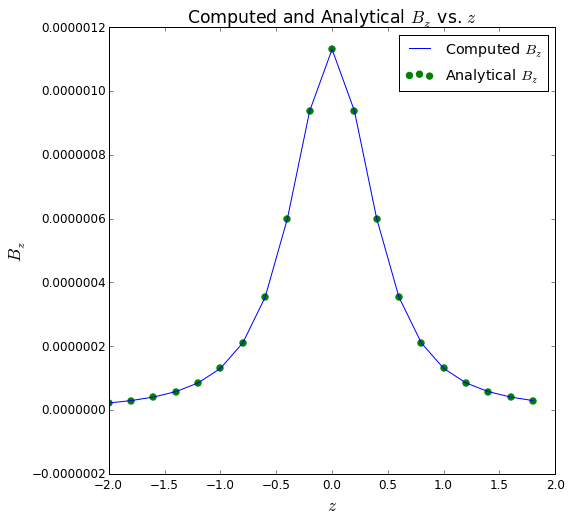
\includegraphics{images/output_19_2.png}
\caption{}
\end{figure}

We see excellent agreement between the numerically computed \(B_z\) and
the analytical \(B_z\) on the \(z\)-axis.

\subsubsection{Exercise 3}\label{exercise-3}

\begin{figure}[htbp]
\centering
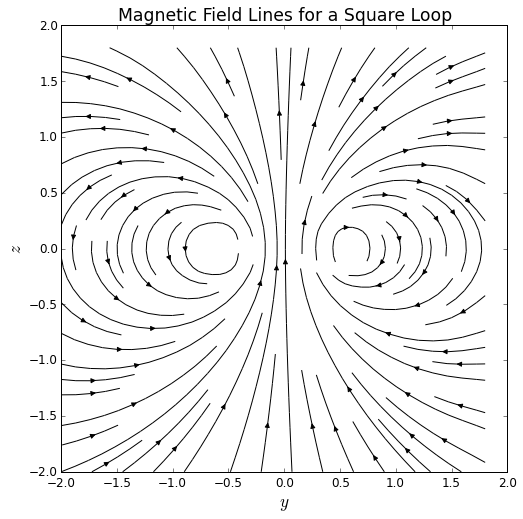
\includegraphics{images/output_15_2.png}
\caption{}
\end{figure}

As we expect for a loop of wire, we see a magnetic field pattern that
resembles that of a dipole field outside of the loop. Inside the loop,
we see that the magnetic field is, indeed, strongest at points near the
wire itself. This exercise can be used to emphasize the relationship
between the density of magnetic field lines and the strength of the
magnetic field - the field lines are densest where the magnetic field is
strongest (at points near to the source), and the field lines are
sparser where the magnetic field is weaker (at points farther away from
the source).

\subsubsection{Extension}\label{extension}

As an example of another wire geometry, a helical wire of radius \(R\),
height \(L\), and \(N\) turns is parameterized by
\[ x(t) = R \cos\left( 2\pi N\,t \right), \]
\[ y(t) = R \sin\left( 2\pi N\,t \right), \]
\[ z(t) = Lt - \frac{1}{2}L. \]

In the example below, \(R=1\), \(N=80\), and \(L=2.0\).

\begin{figure}[htbp]
\centering
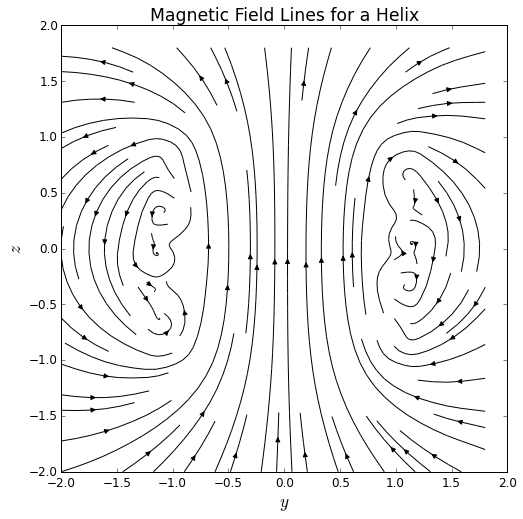
\includegraphics{images/output_26_2.png}
\caption{}
\end{figure}

Because this helix is a simple approximation of a solenoid, we do see
the magnetic field become nearly uniform inside the helix. From the
density of the field lines, the magnetic field is also seen to be much
stronger inside the helix than outside. Outside of the helix, we see the
magnetic field begin to resemble the magnetic field of a dipole, as it
should.

\subsection{Connections to Physics
Texts}\label{connections-to-physics-texts}

D. J. Griffiths, \emph{Introduction to Electrodynamics}, Chapter 5.

\end{document}
